%\title{Processing BTS Booklists Through the POS System}
\documentclass[a4paper, 12pt]{article}
\usepackage{graphicx, subcaption, amsmath, xcolor, geometry, fontspec, atbegshi}
\geometry{margin=1.0in}
\usepackage[os=win]{menukeys}
\AtBeginDocument{\AtBeginShipoutNext{\AtBeginShipoutDiscard}}

\newfontfamily\headingfont{Gill-Sans-MT-Condensed}[
    Path = ./fonts/,
    Extension = .TTF,
    UprightFont=*,
    Scale = 3
]
\let\Huge\headingfont

\begin{document}
\begin{titlepage}
	\begin{minipage}[t]{1\columnwidth}
		\begin{flushright}
       	\vspace{-0.6in}
       	
\includegraphics[width=0.3\textwidth]{MonextraNew.png}
			\vspace{0.5in}
		\par\end{flushright}
	\end{minipage}

	\begin{center}
		{\Huge Processing BTS Booklists Through the POS System}
	\end{center}
	\vspace{2em}
	\noindent
	\textbf{Created:} January 5, 2024
	\hfill
	\textbf{Updated:} \today
	\\\\\indent
	Following are the steps required to process a BTS booklist that has been 	made up by a staff member when the customer is not present. If the 	customer is present while the booklist is being picked then these steps 	are not neccessary.
	
	\tableofcontents
\end{titlepage}

%\newpage
\section{Creating the Customer Account}
Before ringing up booklist items, you must first create an account for the customer if one does not already exist.

\begin{enumerate}
    \item Press \keys{\esc} to exit the POS screen.
    \item Select \menu{Customer Maintenance} in the third column of options.
    \item Press \menu{Add} in the top bar or \keys{F11} to add a new customer account.
    \item Enter the first three letters of the customers last name into the \textit{Customer Code} box and press \keys{\enter}.
    \item Type the customers full name into the \textit{Customer Name} box.
    \item Keep pressing \keys{\enter} until the \textit{Mobile} box is highlighted and enter the customers mobile number.
    \item Keep pressing \keys{\enter} until the \textit{Zone} dropdown is highlighted and select \menu{Back To School}
    \item Keep pressing \keys{\enter} until the \textit{Salesperson} dropdown is highlighted and select your name.
    \item Keep pressing \keys{\enter} until the \textit{Payment Terms} dropdown is highlighted and select \textit{Immediate}
    \item Press \menu{Save} in the top bar or \keys{F12} to finalise adding the account.
    \item Press \keys{\esc}, then press \menu{TouchPOS} to return the the POS screen.
\end{enumerate}
\begin{figure}[ht]
    \centering
    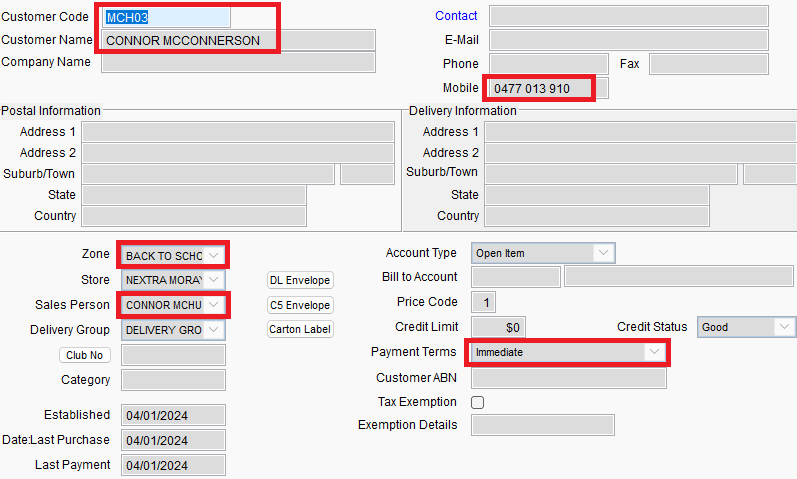
\includegraphics[width=0.8\linewidth]{images/customeraccount.png} 
\end{figure}
The new customer account has now been created.

\clearpage
\newpage
\section{Ringing Items Up to the Customer Account}
Once you have picked all of the items in the book list, you must ring them up to the customer's account. For customers that have multiple booklists, please ring each list up as a separate transaction.

\begin{enumerate}
    \item Press \menu{Customer Lookup} in the function buttons section on the POS screen.
    \begin{figure}[h]
        \centering
        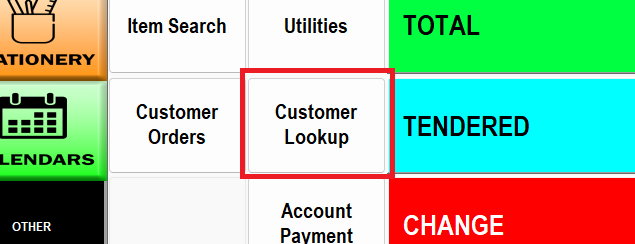
\includegraphics[width=0.5\linewidth]{images/customerlookup.png}
    \end{figure}
    \item Type in the first three letters of the customers last name and use the \keys{\arrowkeyup} and \keys{\arrowkeydown} keys to select the correct customer account and press \keys{\enter}.
    \item Ring up all of the items that you have picked. Check against the list as you are ringing them up to double check that you have the correct items and quantities.
    \item Once everything has been rung in, press \menu{Tender}, a receipt will print.
    \item Log back into the POS screen and press \menu{All Sales}, then press \menu{Reprint Invoice} and print the invoice to the \textit{Front Counter Printer}
    \begin{figure}[h]
    \centering
        \hfill
        \begin{subfigure}{0.4\linewidth}
            \centering
            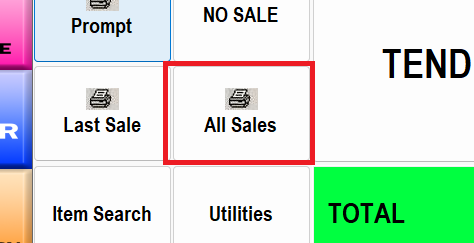
\includegraphics[width=\linewidth]{images/allsales.png}
        \end{subfigure}
        \hfill
        \begin{subfigure}[b]{0.4\linewidth}
            \centering
            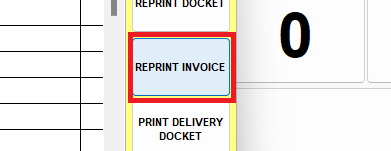
\includegraphics[width=\linewidth]{images/reprintinvoice.png} 
        \end{subfigure}
        \hfill
    \end{figure}
    
    \item Write the year level of the booklist on the bottom on the invoice, and if there are multiple bags, make a note of how many bags there are.
\end{enumerate}

\clearpage
\newpage
\section{Selling the Booklist to the Customer}
When the customer comes in to pick up the booklist, you will need to follow the following steps to finalise the sale. Note: these steps are not necessary if the invoice has a \textit{Paid} stamp on it, if this is the case you can just hand the booklist over to the customer.

\begin{itemize}
    \item Press \menu{Account Payment} in the function buttons section on the POS screen.
    \begin{figure}[h]
        \centering
        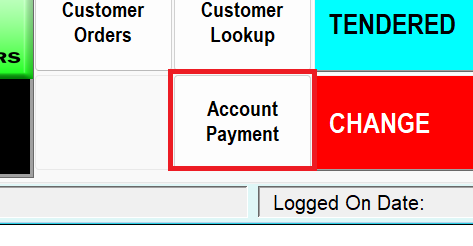
\includegraphics[width=0.3\linewidth]{images/accountpayment.png}
    \end{figure}
    \item Type in the customer code that is on the invoice in the \textit{Customer Code or Invoice No} box and press enter.
    \begin{figure}[h]
        \centering
        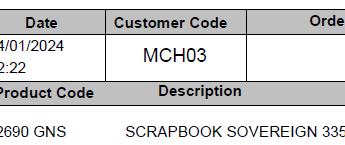
\includegraphics[width=0.3\linewidth]{images/invoicecustomercode.png}
    \end{figure}
    \begin{figure}[h]
        \centering
        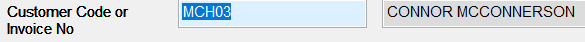
\includegraphics[width=0.7\linewidth]{images/accountcode.png}
    \end{figure}
    \item Press \menu{Alter} in the top bar or \keys{F10} to enter alter mode on the customers account.
    \item Press the \menu{Statement Date} button, you will see that the \textit{Total} will update to the total of any booklists that have been rung up on the customers account.
    \begin{figure}[h!]
        \centering
        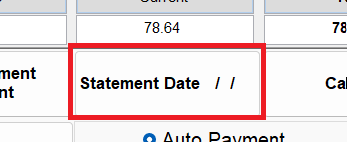
\includegraphics[width=0.3\linewidth]{images/statementdate.png} 
    \end{figure}
    \item Press \menu{Tender in POS} to bring the transaction back to the POS screen and finalise the transaction as normal.
    \begin{figure}[h!]
        \centering
        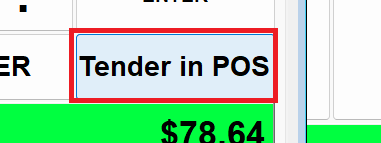
\includegraphics[width=0.3\linewidth]{images/tenderinpos.png}
    \end{figure}
\end{itemize}

\end{document}
